\chapter{Orbiter}

\section{Orbital Parameters}

\section{Design}

\subsection{Instruments}

* Telescope

\autsubsection{Radiation Shielding Theory}{Jean-Paul Breuer}
With regards to the instrumentation on board, there will need to be some type of shielding as protection against harmful radiation as well as from the potential heat generated by the RTG. Whenever gamma radiation passes through matter, it undergoes absorption via Compton, photoelectric, and pair-production interactions. Therefore, the intensity of the emitted radiation decreases as a function of thickness and density of the absorbing material, as stated by the Beer-Lambert law,
\begin{equation}
I = I_0 e^{-\alpha x}
\end{equation}

rearranging the relation and taking the log of both sides gives,\\
\begin{equation}
\ln\left( \frac{l_0}{l}\right) = \alpha x
\end{equation}

where then finding the half value layer (HVL), or where the initial intensity is halfed, can be computed through,\\
\begin{equation}
\ln(2) = \alpha x_{1/2} \Rightarrow x_{1/2} = \frac{0.693}{\alpha} \label{halfthickness}
\end{equation}
In other words, the more dense the material, the less thickness will be required to effectively attenuate the radiation. However, as mentioned previously, whenever radiation passes through matter, there are several interactions that can occur, including X-ray fluorescence.

The transition energy between two electron shells within an atom (typically higher shells K,L,M,+) is the same as the energy of characteristic radiation for that element, which manifests itself as the inner-shell ionization by an accelerated electron. Naturally, ionization can occur in several different electron levels, forming a characteristic spectrum for each element, since all transition energies are unique to each atom. This transition of an excited atom into a lower energy occurs via the photoelectric effect, where radiation ejects inner shell electrons, whereby electrons from the outer shells are transfered into the inner shells to fill in the vacancies, emitting a photon in the X-ray range that is unique to that element with energy equal to the transition energy $E_c = E_m - E_n$. This is the case for elements with higher atomic numbers; however, for elements with low atomic numbers, the Auger effect tends to dominate, where instead of the energy being emitted as a photon, it instead is transfered to another electron which is then ejected from the atom.

The empirical law for the characteristic X-ray emission from an atom is given by Moseley's Law,\\
\begin{equation}
E_c= R_h \cdot (Z-\sigma)^2 \left(\frac{1}{n^2} - \frac{1}{m^2}\right)\label{moseley:eq}
\end{equation}

where $R_h$ is the Rydberg constant, $Z$ is the atomic number, and $\sigma$ is the screening constant of the atom. It is then possible to estimate the energy of a $K_\alpha$ transition via the relation,\\
\begin{equation}
E_{K_\alpha} = A \cdot (Z-1)^2 \label{transition}
\end{equation}
where $A = 10.22$ eV is the $K_\alpha$ transition in hydrogen. Following Equation \ref{transition}, it is evident that every element has its own characteristic fingerprint, but more importantly, to create an effective shielding, it will be required to use several layers with different materials, to gradually attenuate all of the energy to a point where it will no longer damage the sensitive instrumentation. Given that the Orbiter will be orbiting Jupiter, with a heavy radiation environment, it will be very important to minimize the radiation as much as possible, especially during the Lander phase of the mission when the equipment will be most exposed to the harmful radiation from the planet.

\subsection{Thermal design}

\section{Determination of Landing Site}

\autsubsection{Image Recognition}{Kristian Sloth Lauszus}

Since the bandwidth from the orbiter to the earth is limited it is beneficial to have a semi-autonomous system that can pick an potential landing site from some given parameters. For instance it would be useful to pick a landing site that does not have any ridges, as there is risk of the lander tipping over after the landing. This could be done by simple edge detection, such as a Laplacian Gaussian filter from a greyscale image. If the system finds a potential landing site the image could then be streamed back to earth either as a binary, greyscale or even the full color image for further analysis. Furthermore object detection could be used to locate certain characteristics. The image could then be cropped and streamed back to earth, thus decreasing the needed bandwidth.

Figure \ref{fig:edge_detection} shows two examples of how a Laplacian Gaussian filter has been used for edge detection on images from the moon. It shows clearly how cracks on the surface show up. These locations could then be picked as potential landing sites and further analysed by the ground control.

\begin{figure}[htb]
	\centering
	\subfloat{
		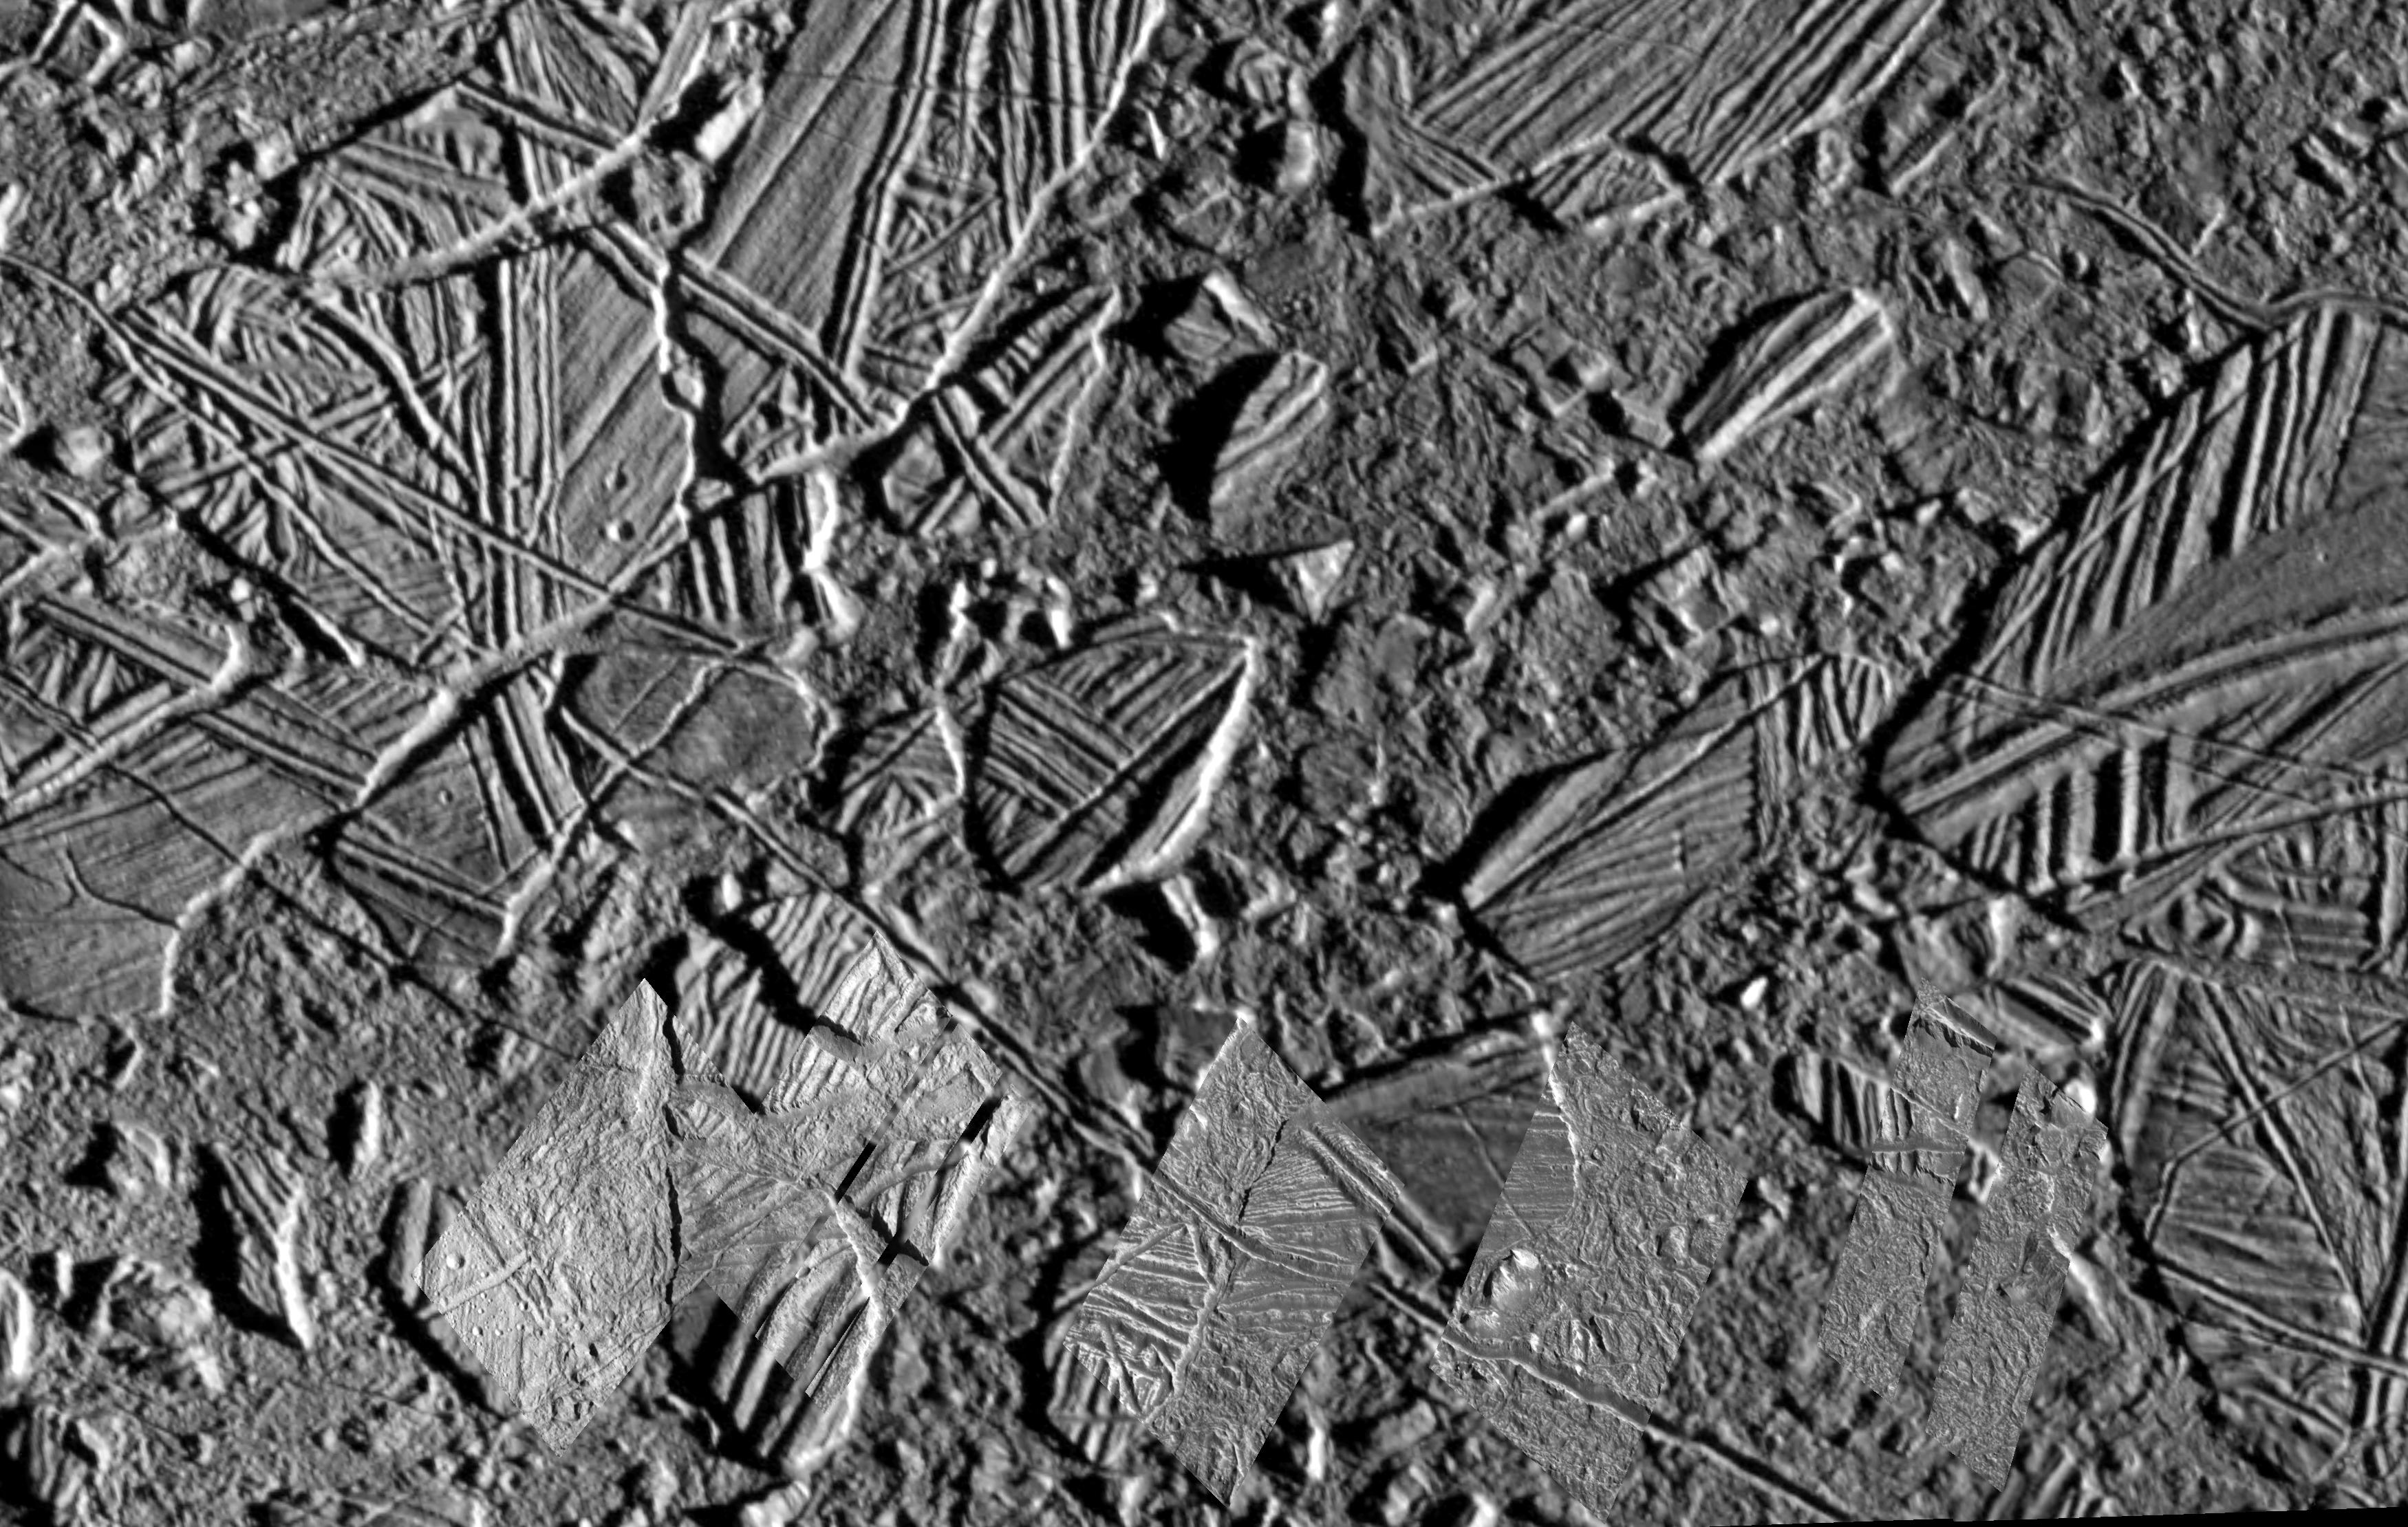
\includegraphics[width=.48\textwidth]{figures/edge/PIA01403}
	}
	\subfloat{
		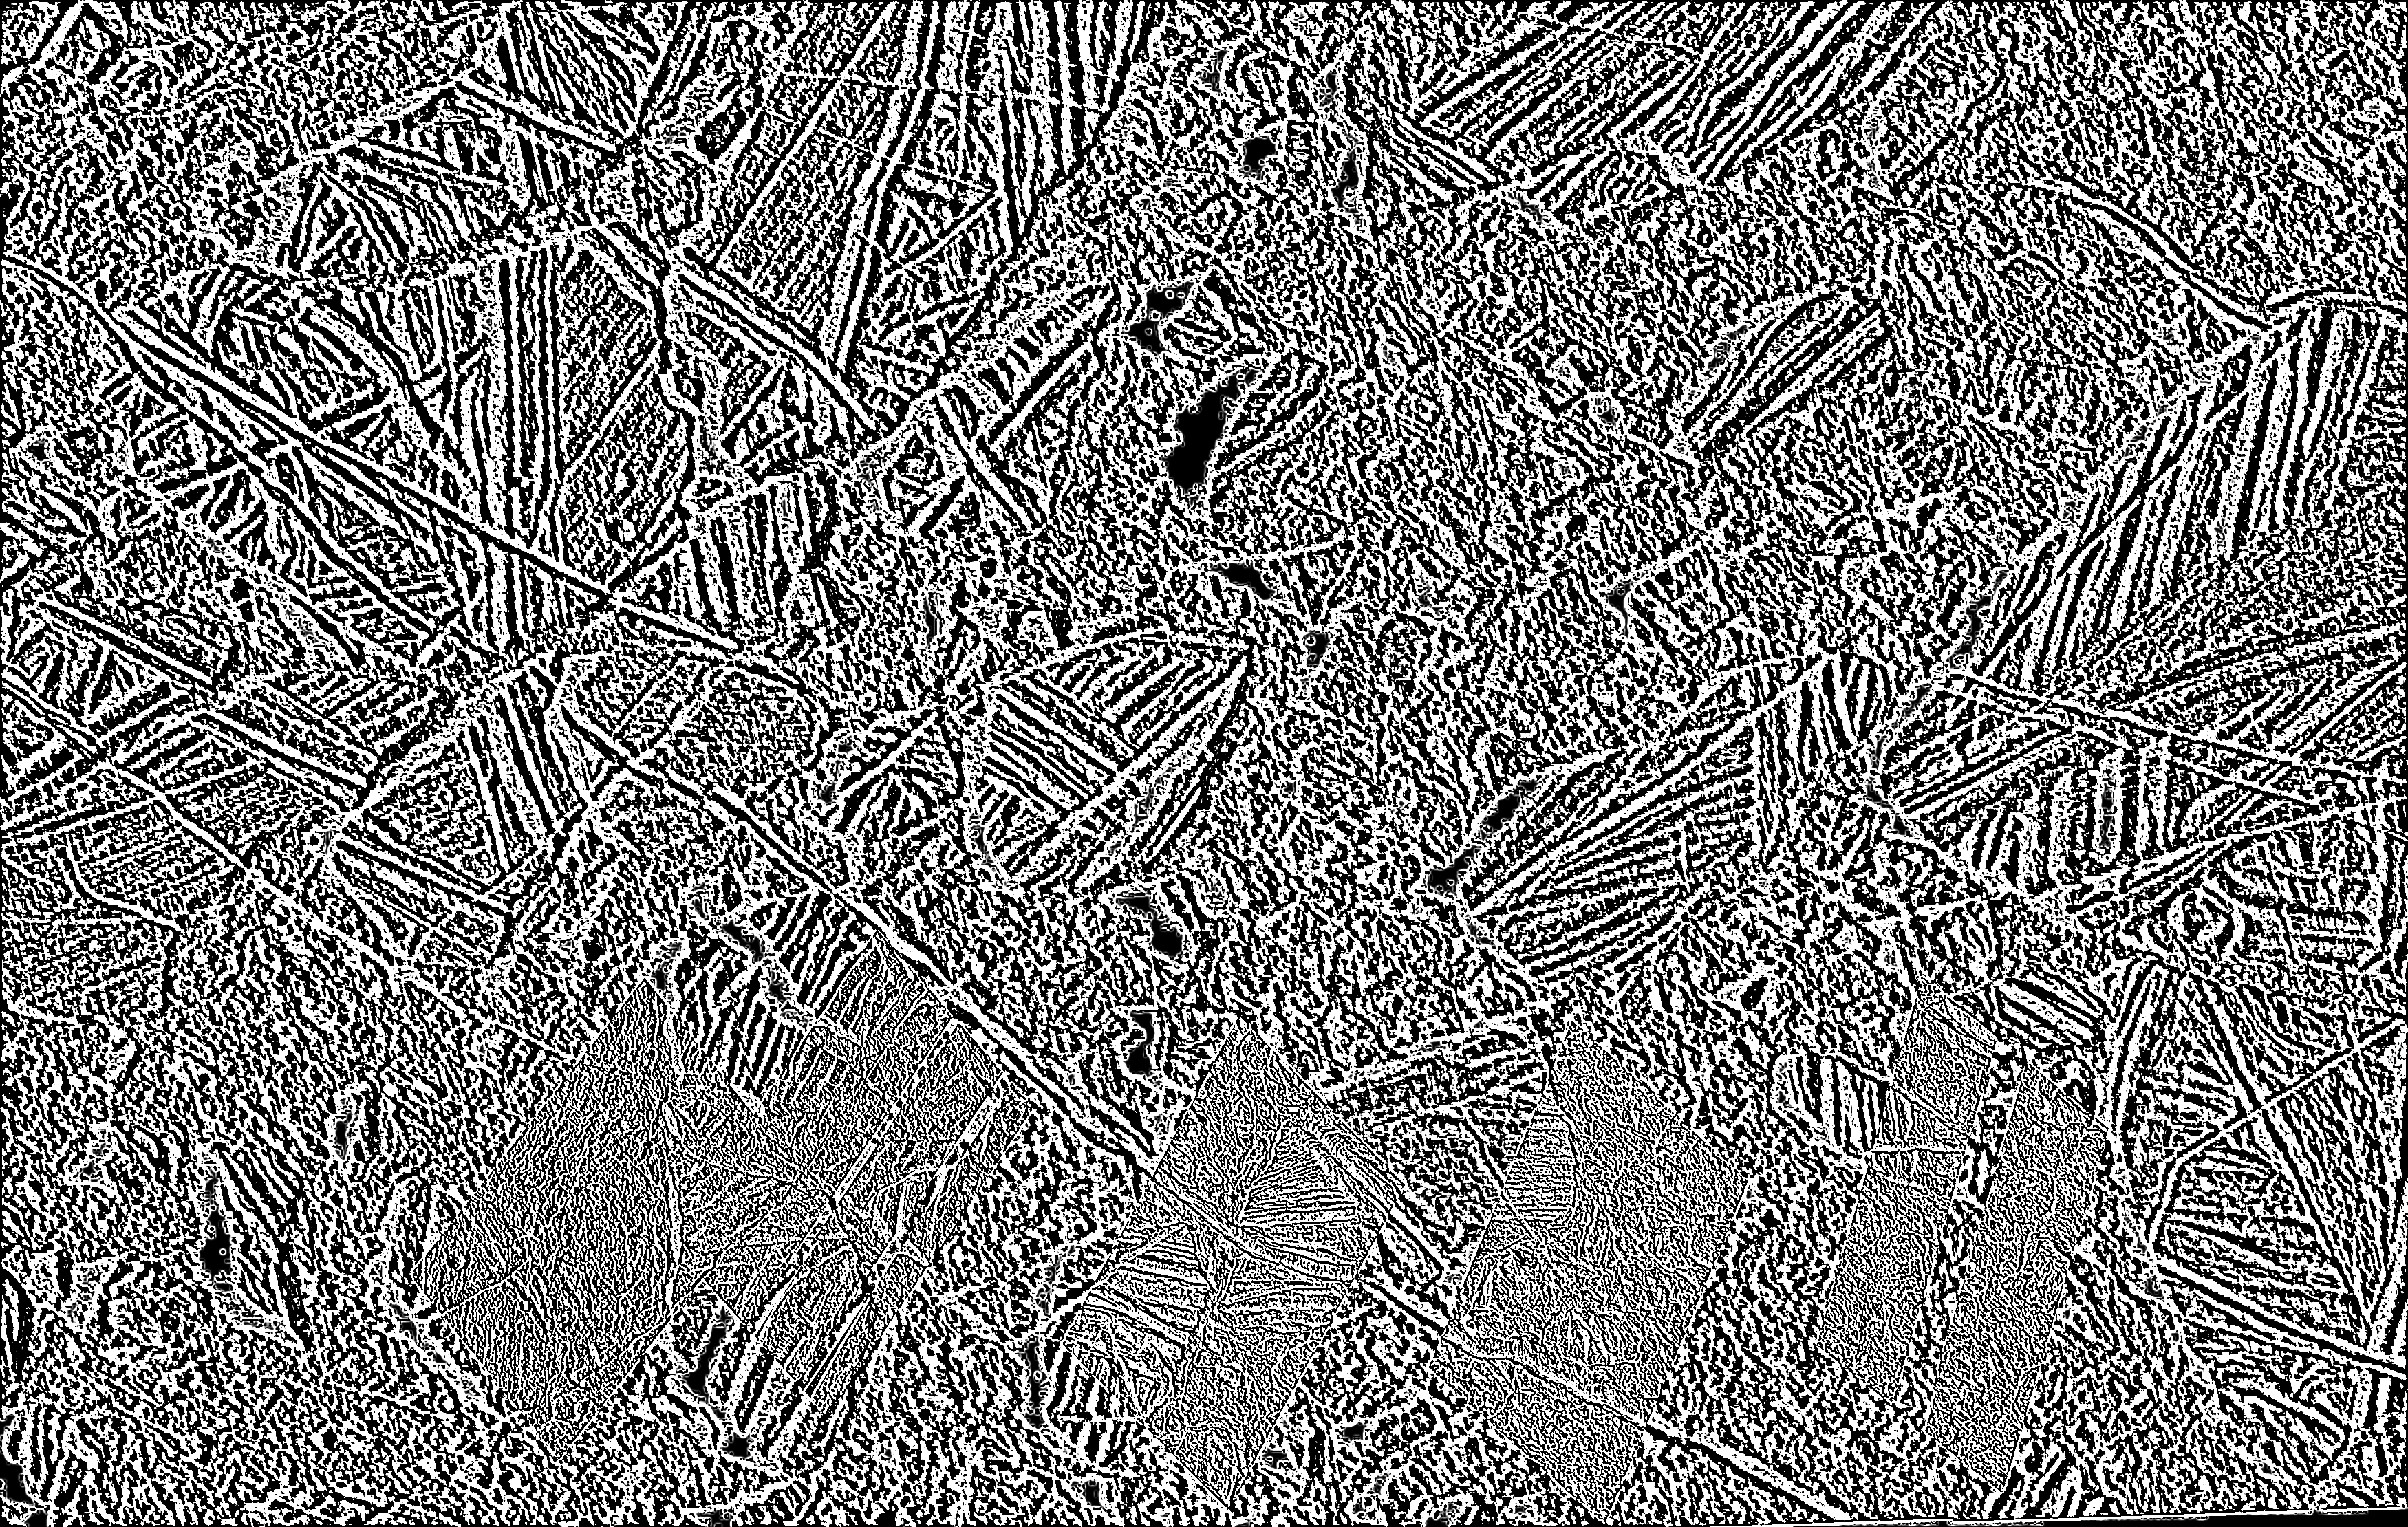
\includegraphics[width=.48\textwidth]{figures/edge/PIA01403_filtered}
	}
	\\
	\subfloat{
		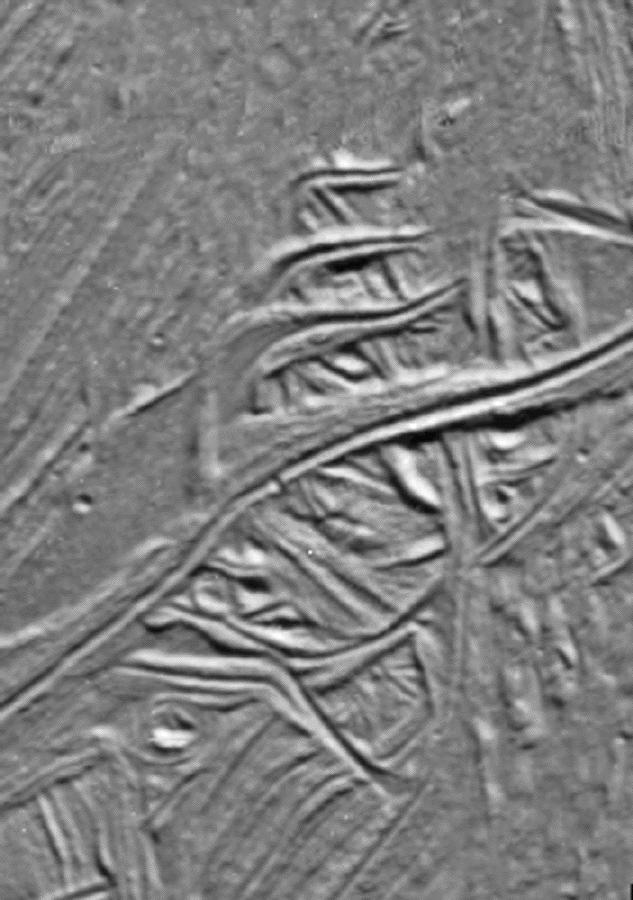
\includegraphics[width=.31\textwidth]{figures/edge/PIA01642}
	}
	\subfloat{
		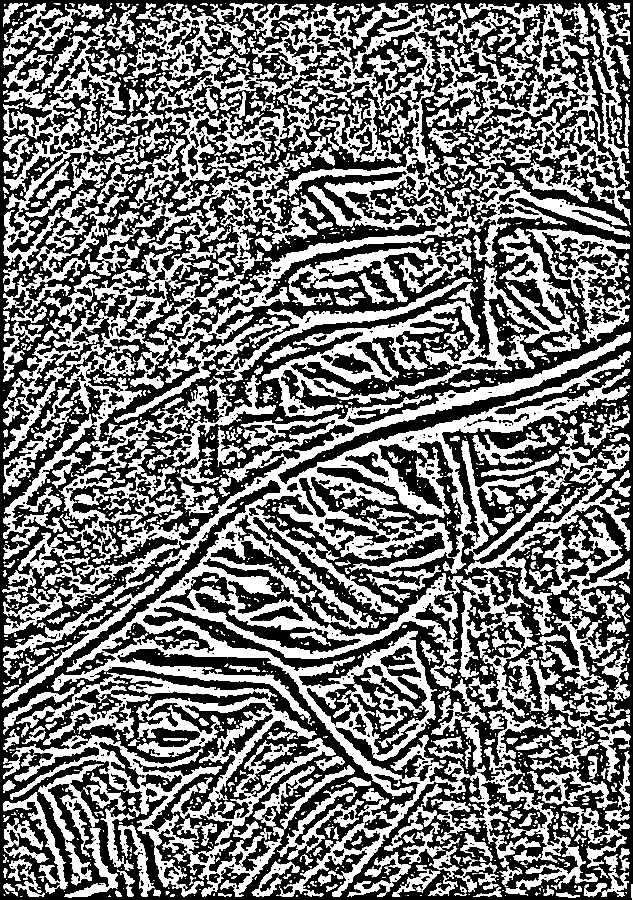
\includegraphics[width=.31\textwidth]{figures/edge/PIA01642_filtered}
	}
	\subfloat{
		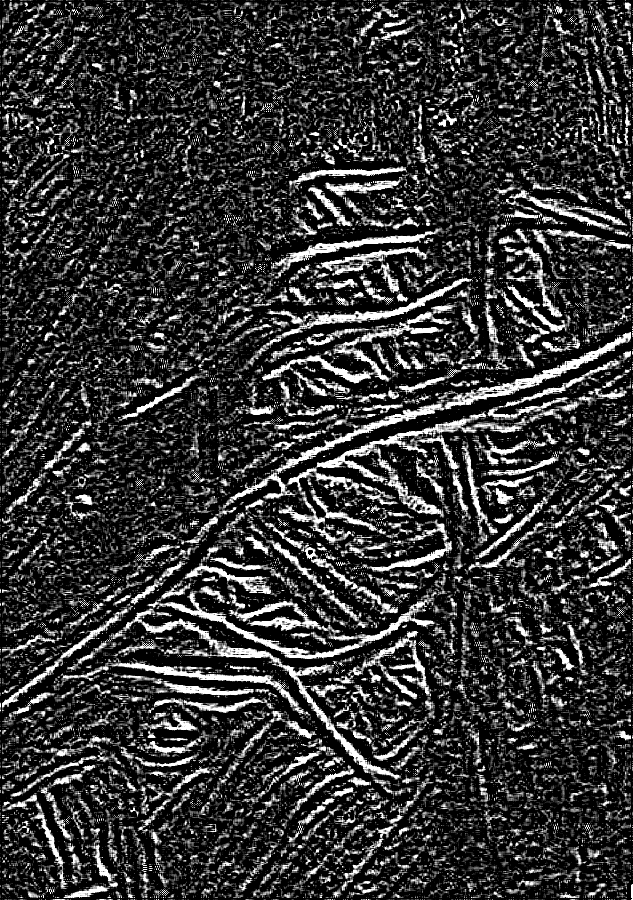
\includegraphics[width=.31\textwidth]{figures/edge/PIA01642_filtered_alternativ}
	}
	\captionsetup{width=.9\textwidth}
	\caption{Example of Laplacian Gaussian filter used for edge detection on the surface of the moon}
	\label{fig:edge_detection}
\end{figure}

\subsection{Mapping of the moon}

\subsection{Europa Coordinate System}

* How to determine the ice thickness?

* Thinnest ice, smooth area, no boulders, avoid craters

* Radiation
